\section{Partie théorique : Programmation sur KEYENCE - principes de base}
\noindent Comme dans beaucoup de langages de programmation, la programmation sur KEYENCE se fait au travers :
\begin{itemize}
\item \textbf{de variables} qui permettent de stocker/restituer des informations,
\item \textbf{de fonctions} qui permettent de faire toutes sortes d’opérations.
\end{itemize}


\subsection{Les variables}
\label{Sec.Variables}

\subsubsection{Catégories et types de variables}
\label{Sec.Variables_CatTypes}
\noindent Les variables sont séparées en plusieurs catégories :
\begin{enumerate}
  \item Les variables \textbf{Locales} qui appartiennent au programme en cours : 
  elles sont donc accessibles uniquement dans le programme en cours,
  \item Les variables \textbf{Globales} qui appartiennent au contrôleur : elles 
  sont donc accessibles à tous les programmes qui tournent sur le contrôleur ; on 
  y stockera exclusivement les variables invariables propres au système et qui ne
  change pas d’un programme à l’autre, comme les résultats de la balance des blancs,
  par exemple,
  \item Les variables \textbf{Image} qui appartiennent aussi au programme en 
  cours : elles sont stockées séparément des ‘variables Locales’ car de par leur taille,
  elles sont traitées différemment, mais elles se comportent de la même manière,
  \item Les variables \textbf{Temporaires} qui appartiennent à un bloc de calcul 
  « Calculation » qui sont instanciées au début de l’exécution du bloc et détruite à
  la fin de ce dernier. Elles ne peuvent donc pas être propagées d’un bloc à l’autre
  et ne servent donc que de variables tampons utiles dans les processus calculatoires
  pour stocker des informations temporaires,
  \item Les variables \textbf{Système} qui appartiennent au contrôleur et qui
  permettent de manipuler le comportement direct de l’automate en activant le 
  Trigger, ou en manipulant des flags BUSY/IDLE du système.
\end{enumerate}

\vspace{0.2cm}

Le langage de programmation KEYENCE étant typé, les variables Locales et Globales peuvent prendre différents types :
\begin{itemize}
  \item \textbf{Numerical :} une simple valeur numérique,
  \item \textbf{Position :} une double valeur numérique des coordonnées d’un point 
  (X et Y),
  \item \textbf{Line :} une double valeur numérique thêta (T) et rho (RH) correspondant 
  à la représentation selon Hough d’une ligne,
  \item \textbf{Circle :} une triple valeur numérique coordonnées du centre (CX et CY) 
  et le rayon (CR),
  \item \textbf{3D Pos :} une triple valeur numérique des coordonnées d’un point (X, Y 
  et Z) en 3D,
  \item \textbf{Plane :} une triple valeur numérique des paramètres définissant un plan 
  en 3D (PPA, PPB et PPC).
\end{itemize}
Chacun de ces types peut être \textbf{simple}, ou sous forme de \textbf{tableau (array)}.


\subsubsection{Les noms de variables}
\label{Sec.Variables_Names}
\noindent Sur les logiciels XG-X, chaque variable est désignée par un préfixe et un 
nom :
\begin{center}
\textit{‘préfixe’’nomDeVariable’}
\end{center}
\noindent Pour le préfixe, chaque catégorie de variable se différenciera dans le code par un préfixe spécifique :
\begin{itemize}
  \item \textbf{'\#'} désigne les variables locales,
  \item \textbf{'\$'} désigne les variables globales,
  \item \textbf{'\&'} désigne les variables images,
  \item \textbf{'@'} désigne les variables temporaires,
  \item \textbf{'!'} désigne les résultats des blocs (expliqué au point 
  ~\ref{Sec.Functions_UnitResults}),
  \item \textbf{'\%'} désigne les variables système.
\end{itemize}
\vspace{0.2cm}

\noindent Pour le nom de la variable, rien à signaler, si ce n’est que :
\begin{itemize}
\item la casse de caractère est respectée,
\item l’usage des ‘\_’ dans les noms est prohibé.
\end{itemize}
\vspace{0.2cm}

\noindent Ainsi, pour créer une variable locale appelée \textit{"maVariable"}, on écrira simplement \textit{"\#maVariable"}.


\subsubsection{Déclarer une variable}
\label{Sec.Variables_Declaration}
Pour déclarer une nouvelle variable, il suffit de cliquer sur l’icône « Variables » (illustré sur l'image ~\ref{fig.Variables_IconLocation}) et une fenêtre s’ouvre avec 3 onglets distincts pour chacune des catégories de variables présentées plus haut. Cette fenêtre est accessible n’importe quand même si d’autres fenêtres sont ouvertes.\\
\vspace{0.2cm}

\noindent
\begin{minipage}[c]{\textwidth}
  \centering
  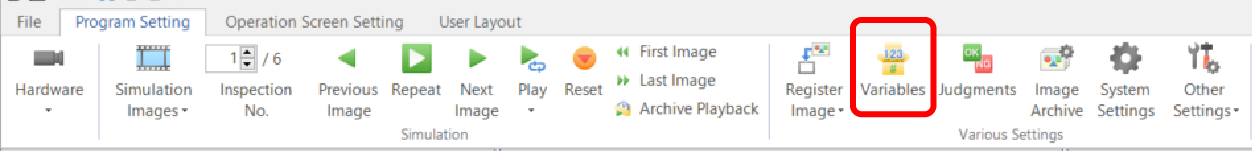
\includegraphics[width=16cm, height=10cm, keepaspectratio]{addOns/LaboCalib_Variables_Icon.png}
  \captionof{figure}{\textit{Localisation de l’icone Variables}}
  \label{fig.Variables_IconLocation}
\end{minipage}\\
\vspace{0.2cm}

\noindent
\begin{minipage}[c]{\textwidth}
  \centering
  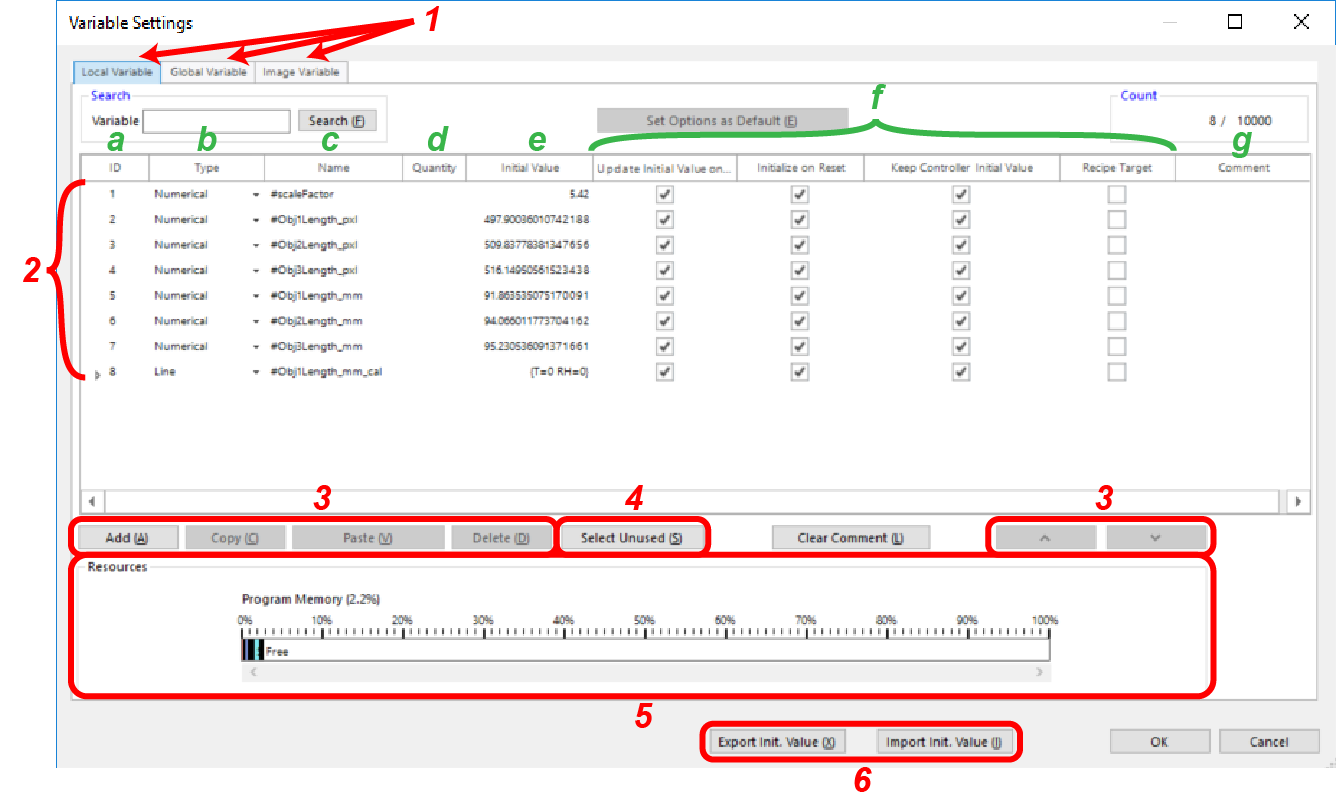
\includegraphics[width=16cm, height=10cm, keepaspectratio]{addOns/LaboCalib_Variables_Window.png}
  \captionof{figure}{\textit{Fenêtre de gestion des variables}}
  \label{fig.Variables_Window}
\end{minipage}\\
\vspace{0.2cm}

\noindent Cette fenêtre présente \footnote{Les numéros de la liste ci-dessous
correspondent aux indices sur l'image ~\ref{fig.Variables_Window}} :
\begin{enumerate}
  \item un onglet par catégorie de variables,
  \item pour chaque catégorie de variable, la liste de toutes les variables de cette
  catégorie, avec pour chaque variable :
  \begin{enumerate}
    \item son ID,
    \item son type,
    \item son nom,
    \item la quantité d’éléments contenus dans cette variable (quand la variable est 
    un tableau),
	\item sa valeur initiale,
	\item divers flags,
    \item un commentaire pour la décrire.  
  \end{enumerate}

  \item des boutons pour ajouter/copier/coller/supprimer/réorganiser l’ordre des
  variables,
   \item un bouton pour trouver toutes les variables inutilisées dans le code,
   \item un affichage de l’utilisation de la mémoire que ces variables occupent,
   \item des boutons pour importer/exporter les valeurs initiales des différentes
   variables du programme.
\end{enumerate}
\vspace{0.2cm}


\noindent Une fois que cette fenêtre est ouverte, il faut :
\begin{enumerate}
  \item cliquer sur le bouton ajouter,
  \item entrer un nom de variable (si aucun préfixe n’est spécifié, le software 
  le préfixera automatiquement le nom en fonction de la catégorie choisie),
  \item entrer une valeur initiale.
\end{enumerate}
\vspace{0.2cm}

\noindent
\textcolor{red}{\textbf{Attention 1 :} veillez à toujours déclarer vos variables en local !}
\vspace{0.2cm}

\noindent
\textbf{Attention 2 :} Toutes les variables sont créées à l’appel du programme et ne sont détruites que lorsque le programme est quitté (suite à une extinction du système ou un changement de programme, par exemple). Cela qui signifie que les variables sont conservées (avec leur valeur) à la fin de l’exécution du programme suite à un Trigger, et lancer un nouveau Trigger ne réinitialisera pas les variables. De plus, par défaut, le flag « overwrite initial value on save » des variables est activé, ce qui permet au programme d’enregistrer les valeurs actuelles des variables comme valeurs initiales futures. Pensez à désactiver cette fonction, si ce n’est pas ce que vous désirez !\\


\subsubsection{Accéder à/allouer une variable}
\label{Sec.Variables_Allocation}
Une fois que la variable est déclarée dans la fenêtre « Variables », elle 
est créée et instanciée dans tout le programme et est donc appelable dans tout le code
(comme dans des blocs de calcul "Calculation", par exemple, ou encore comme 
paramètre de blocs fonctionnels \textit{illustré sur le bas de l'image 
~\ref{fig.Functions_UnitResults}}).

Pour appeler la variable, il faut simplement écrire son nom comme spécifié dans le paragraphe ~\ref{Sec.Variables_CatTypes} et le tour est joué. Ensuite, d’une manière générale, l’accès au différents champs d’une structure ou éléments d’un tableau se fait \textbf{comme dans le langage C} :
\begin{itemize}
  \item Pour une \textbf{structure}, l’accès à chaque champ se fait avec un '.' . Par
  exemple, pour accéder à la coordonnée X d’une variable globale de position appelée
  \textit{"maPosition"}, on écrira \textit{"\$maPosition.X"},
  \item Pour un \textbf{tableau}, l’accès à chaque élément du tableau se fait avec 
  des crochets, les indices vont de 0 à $taille_{tableau} – 1$. Par exemple, pour
  accéder à la 3ème case du tableau local \textit{\#positionsDesPoints}, on écrira
  \textit{"\#positionsDesPoints[2]"}.
\end{itemize}


\subsubsection{Astuce -- l'outil d'auto-complétion}
\label{Sec.Variables_AutoComplete}
XG-X VisionEditor possède un système d’auto-complétion efficace qui propose
automatiquement toutes les variables disponibles. Par exemple, une variable globale
position appelée \textit{"\$firstPosition"} est déclarée, en écrivant '\$',
VisionEditor proposera toutes les variables globales, dont celle-ci, puis une fois 
que \textit{"firstPosition"} est sélectionné, si un '.' est ajouté, VisionEditor
proposera automatiquement tous les champs disponibles.



\subsection{Les fonctions}
\label{Sec.Functions}
Les fonctions dans le contrôleurs XG sont toutes encapsulées dans des blocs
fonctionnels. Le matériel KEYENCE offre des fonctions performantes de haut niveau,
facilement et grandement paramétrables qui couvrent pratiquement tous les besoins liés
à la vision industrielle. Pour ajouter une fonction, il suffit donc d’ajouter un bloc
de plus à votre programme, de régler ses paramètres, et rien de plus.


\subsubsection{Paramétrer le bloc}
\label{Sec.Functions_InputParameters}
Lorsqu’une fonction est rajoutée au code, la fenêtre de paramètre s’ouvre automatiquement et donne accès à tous les paramètres de la fonction répartis sur plusieurs onglets.
Le premier onglet est toujours l’onglet "General" qui regroupe des informations descriptives sur le bloc, telles que :
\begin{itemize}
  \item son type de fonction qu’il exécute,
  \item son ID,
  \item son nom\footnote{Prenez l’habitude de nommer vos blocs de manière précise et intelligente et de brièvement commenter le comportement attendu de vos blocs. },
  \item son flag d’exécution,
  \item un espace commentaire.
\end{itemize}
\noindent Certains blocs possèdent d’autres informations sur cet onglet, comme la
variable image d’entrée, par exemple, mais tous ces paramètres sont ajustables sur 
les onglets suivants.
\vspace{0.2cm}

Comme décrit plus haut, les différents onglets permettent de paramétrer la fonction. 
Il existe plusieurs cas de figure pour paramétrer un élément :
\begin{itemize}
  \item avec des valeurs \textbf{fixes} avec un seul champ à remplir,
  \item avec des valeurs \textbf{variables} avec 2 champs à remplir et une case à
  cocher.
\end{itemize}
\vspace{0.3cm}

\noindent
\begin{minipage}[c]{\textwidth}
  \centering
  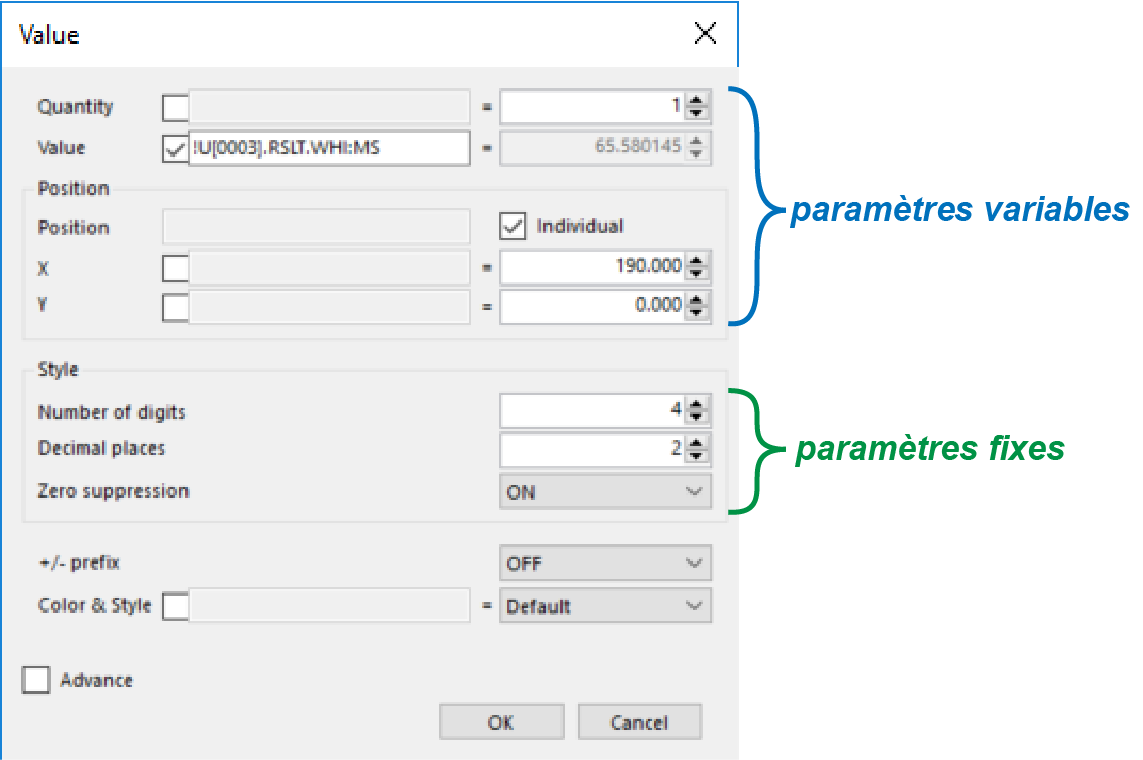
\includegraphics[width=16cm, height=10cm, keepaspectratio]{addOns/LaboCalib_Function_ParametersTypes.png}
  \captionof{figure}{\textit{Types de paramètres de blocs}}
  \label{fig.Functions_ParametersType}
\end{minipage}\\
\vspace{0.3cm}

Certains paramètres possèdent le champ « current value » : lors du paramétrage du bloc, il est possible de Trigger/Run le programme pour voir son comportement et afficher la valeur de ce paramètre, comme pour ajuster les limites admissibles, par exemple.

\noindent
\begin{minipage}[c]{\textwidth}
  \centering
  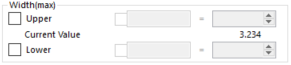
\includegraphics[width=10cm, height=10cm, keepaspectratio]{addOns/LaboCalib_currentValue.png}
  \captionof{figure}{\textit{Champ 'Current value'}}
  \label{fig.Functions_CurrentValue}
\end{minipage}\\
\vspace{0.3cm}


\subsubsection{Accéder aux résultats du bloc}
\label{Sec.Functions_UnitResults}
Lors de leur exécution, chaque bloc génère une série de résultats qui décrivent les résultats intermédiaires et finaux de son exécution. Ils se rangent dans plusieurs catégories :
\begin{itemize}
  \item les résultats de Jugement qui correspondent à un OK/NOK du bloc (ou d’une
  partie du bloc),
  \item les résultats de valeur absolue qui est ce que le bloc de fonction a mesuré
  dans le référentiel de sa caméra,
  \item les résultats de valeur mesurée qui est la valeur absolue mais rapporté dans 
  le référentiel de l’objet à mesurer.
\end{itemize}
\noindent qui sont accessibles depuis la fenêtre Unit Result, sous l’onglet « Unit Result » et affiche les résultats résumés ou les résultats détaillés du bloc (comme illustré sur l’image ~\ref{fig.Functions_UnitResults}).

\vspace{0.2cm}
Tous les résultats détaillés sont stockés dans une structure nommée « RSLT » stockée dans la structure du bloc de fonction. Comme les variables normales, cette structure et donc ses sous-résultats sont accessibles depuis n’importe où dans le code (comme illustré sur l’image ~\ref{fig.Functions_UnitResults}).

\noindent
\begin{minipage}[c]{\textwidth}
  \centering
  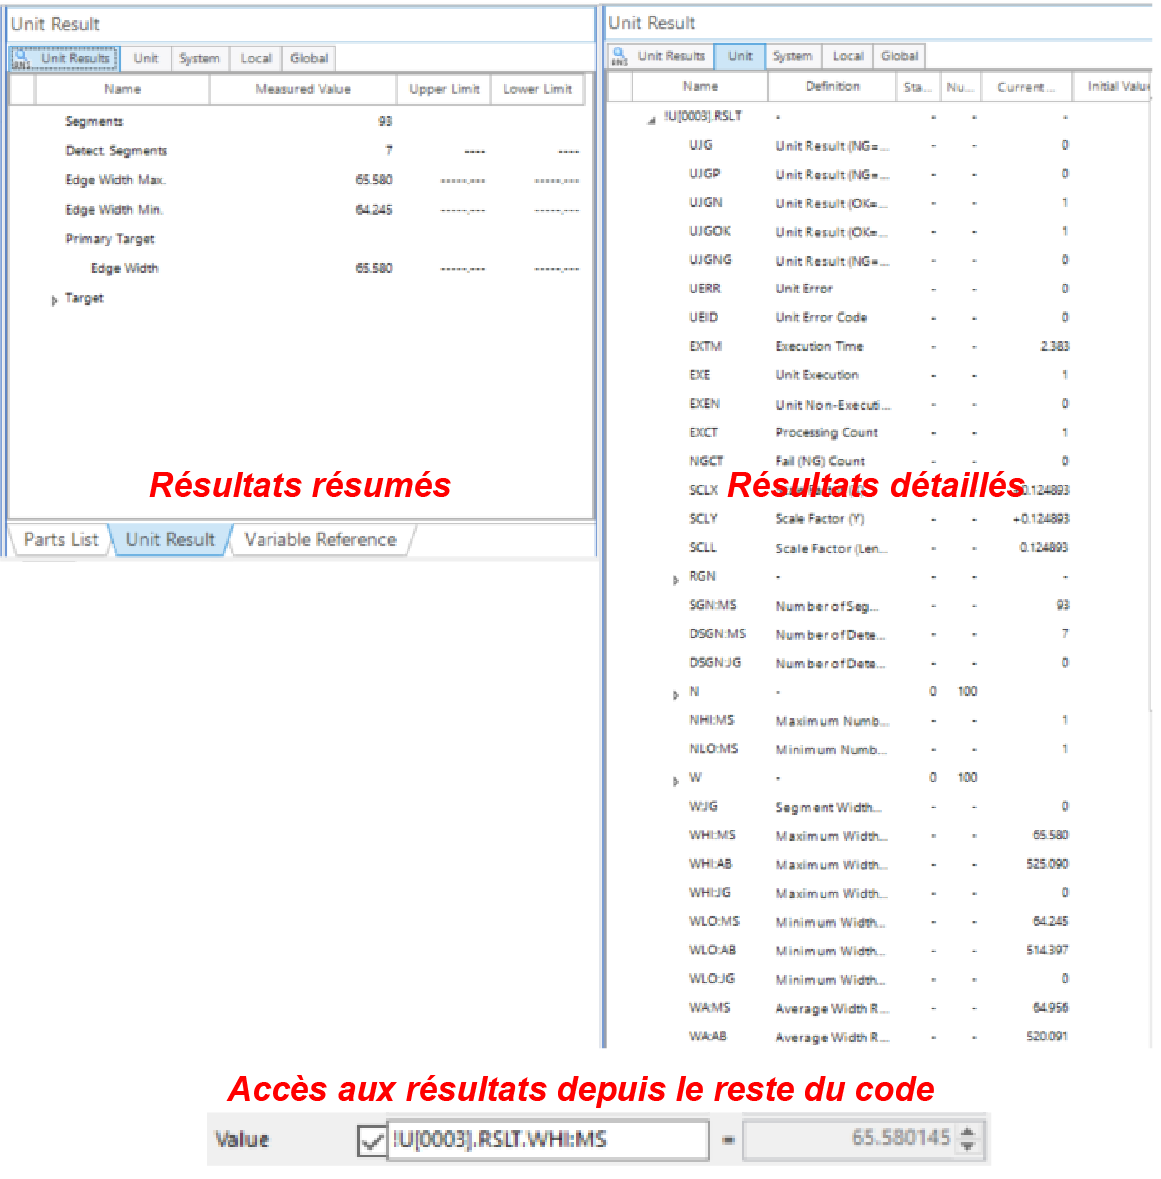
\includegraphics[width=16cm, height=16cm, keepaspectratio]{addOns/LaboCalib_Functions_AccessResult.png}
  \captionof{figure}{\textit{Accès aux différents résultats de l'unité}}
  \label{fig.Functions_UnitResults}
\end{minipage}\\
\vspace{0.3cm}


\subsection{L'utilisation des images par le contrôleur XG}
\label{Sec.Images}
\noindent Les contrôleurs XG manipulent 2 types d’images :
\begin{itemize}
  \item \textbf{les images capturées} sont celles qui sont fournies par la caméra et
  sont soumises à un traitement (mesures/traitement d’image/etc…). Elles sont 
  ‘prises’ au début du trigger au moment où le bloc « capture » est appelé, puis
  manipulées traitées tout au long du processus pour être supprimée à la fin, si 
  aucune autre instruction n’est donnée. Ces images capturées sont stockées dans des
  variables images,
  \item \textbf{Les images de références} sont des images qui servent de référence
  (d’où leur   nom) pour des opérations/calculs tels que la calibration, le pattern
  matching, ou  encore comme base de donnée de caractères pour la lecture OCR. Elles
  sont enregistrées directement dans le contrôleur dans un tableau au moment de la 
  création/édition du programme et \textbf{existent dès le début du programme} et 
  \textbf{ne sont pas supprimées à la fin de l’exécution du programme}. Elles sont 
  inaccessibles en tant que « variable » directement, mais il est possible d’y accéder
  par l’onglet « Image » de tous les blocs qui nécessitent une image de référence.
\end{itemize}


\subsubsection{Images de simulation}
\label{Sec.Images_ImagesTypes}
Lorsque le contrôleur fonctionne, les images capturées sont celles envoyées par la caméra. Mais lors du développement sur un PC sur VisionEditor, aucune caméra ne vient alimenter les blocs capture. C’est possible de simuler cela – c’est pour cela qu’on parle d’’images de simulation’ – grâce à la fenêtre ‘Simulation images’ (ouverte en appuyant sur l'icône éponyme illustré sur l'image ~\ref{fig.Image_SimulationTools} où on peut glisser et déposer toutes les images que l’on souhaite faire passer dans le programme.

\vspace{0.2cm}
Chacun des blocs de capture possède une liste de slots dans lequel on peut glisser des images. Pour que les images soient valides, il faut que les images soient au \textbf{format '.bmp'} et aient \textbf{exactement la même dimension que la variable image dans laquelle elles seront stockées}. Pour chaque image valide, une miniature apparait dans la liste. Pour valider la saisie, il suffit de cliquer sur le bouton OK.

\vspace{0.2cm}
Une fois les images insérées, les boutons de la section « Simulation » permettent de simuler le Trigger du programme :

\begin{enumerate}
  \item Indique l’indice dans la liste de l’image ‘actuelle’ qui sera la prochaine 
  à être insérée dans le programme,
  \item Trigge le programme avec l’image actuelle, 
  \item Trigge le programme avec l’image suivante ou précédente dans la liste,
  \item Passe en boucle toutes les images contenues dans la liste des images de simulation. 
\end{enumerate}
\vspace{0.3cm}

\noindent
\begin{minipage}[c]{\textwidth}
  \centering
  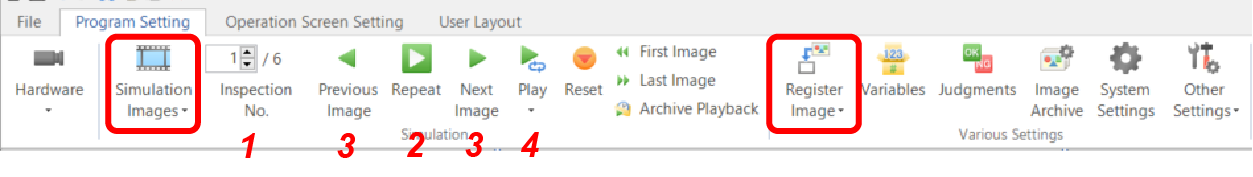
\includegraphics[width=16cm, height=10cm, keepaspectratio]{addOns/LaboCalib_SimulationTrigger.png}
  \captionof{figure}{\textit{Outil de gestion du Trigger en mode Simulation}}
  \label{fig.Image_SimulationTools}
\end{minipage}\\


\subsubsection{Images de référence}
\label{Sec.Images_ReferenceImages}
Chacun des blocs nécessitant une image de référence possède un onglet de paramètres dans lequel il sera possible de spécifier la variable image sur laquelle la variable de référence sera calquée et le numéro de la variable de référence. Attention : ce numéro doit pointé sur une variable de taille et de type cohérents avec l'image poitnée par la variable spécifiée dans « Image Variable ».\\

\noindent
\begin{minipage}[c]{\textwidth}
  \centering
  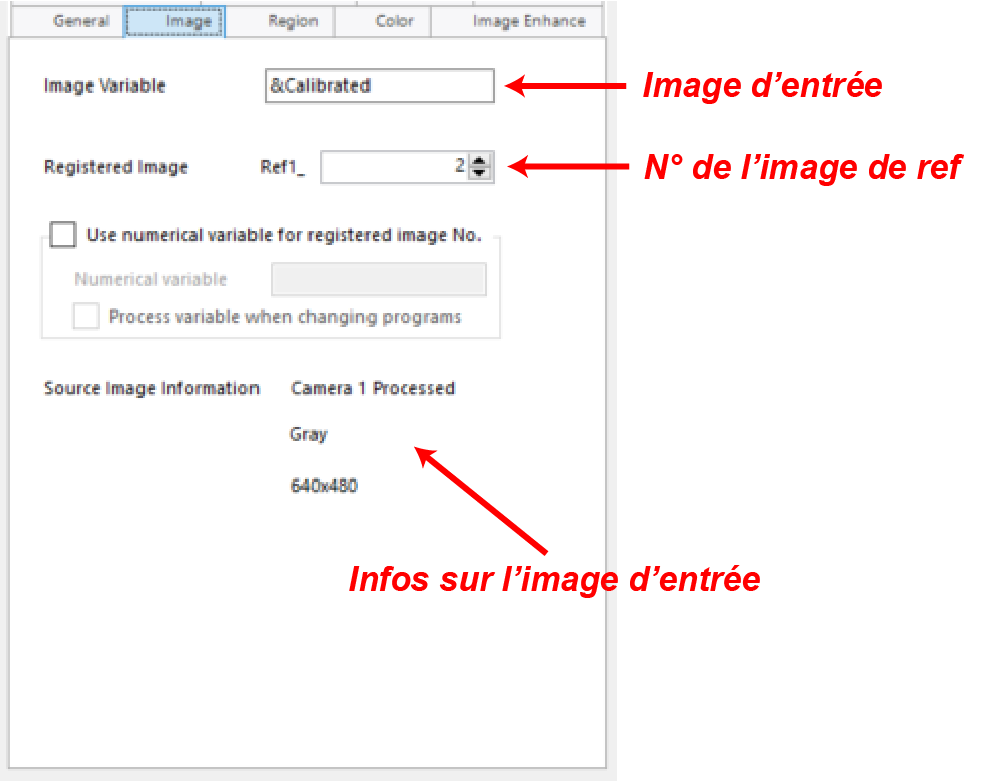
\includegraphics[width=16cm, height=10cm, keepaspectratio]{addOns/LaboCalib_RefImageUnitParameters.png}
  \captionof{figure}{\textit{Entrer une image de référence comme paramètre}}
  \label{fig.Image_RefImages}
\end{minipage}\\
\vspace{0.3cm}

Une fois ce paramètre introduit, le bloc calcule et travaille sur l'image de référence spécifiée. Pour faire commuter sur une image capturée, il suffit de modifier l'image traitée de "Reference Image" à "Captured Image".\\

\noindent
\begin{minipage}[c]{\textwidth}
  \centering
  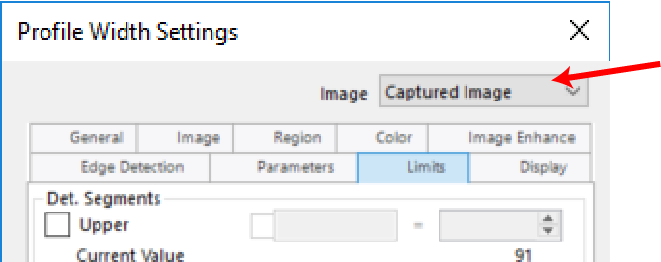
\includegraphics[width=8cm, height=8cm, keepaspectratio]{addOns/LaboCalib_RefImageSwitch.png}
  \captionof{figure}{\textit{Commuter le traitement entre l'image de référence et l'image capturée}}
  \label{fig.Image_RefImagesSwitch}
\end{minipage}\\
\vspace{0.3cm}

Pour enregistrer une image de référence, il suffit simplement à tout moment de cliquer sur le bouton "Register Image" (illustré sur l'image ~\ref{fig.Image_SimulationTools}) et une fenêtre s’ouvre pour nous permettre d’enregistrer une image actuellement dans le processus (traîtée ou non). 

\noindent
\begin{minipage}[c]{\textwidth}
  \centering
  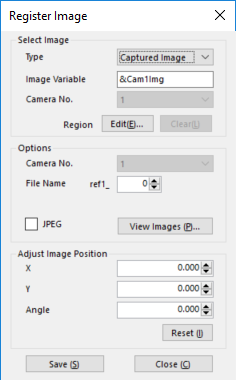
\includegraphics[width=16cm, height=10cm, keepaspectratio]{addOns/registerImage.png}
  \captionof{figure}{\textit{Enregistrer une image de reference}}
  \label{fig.Image_RefImagesSaves}
\end{minipage}\\

Cette fenêtre permet de spécifier :
\begin{itemize}
  \item \textbf{Type} : type d’image (référence/capture/fichier) à enregistrer,
  \item \textbf{Image Variable} : nom de la variable contenant l’image à enregistrer,
  \item \textbf{Camera No.} : le numéro de la caméra d’où vient l’image de référence,
  \item \textbf{Region} : la région de l’image à enregistrer,
  \item \textbf{File Name} : le numéro/nom que l’image enregistrée aura,
  \item \textbf{JPEG} : active la compression des images au format JPEG (utile lorsque la place est limitée),
  \item \textbf{View Images} : affiche toutes les images de référence enregistrées dans le contrôleur pour ce programme,
  \item \textbf{Adjust Image Position} : ajuste la position/orientation de l’image à enregistrer.

\end{itemize}
